% !TEX root = ../../thesis.tex

\cleartoleftpage
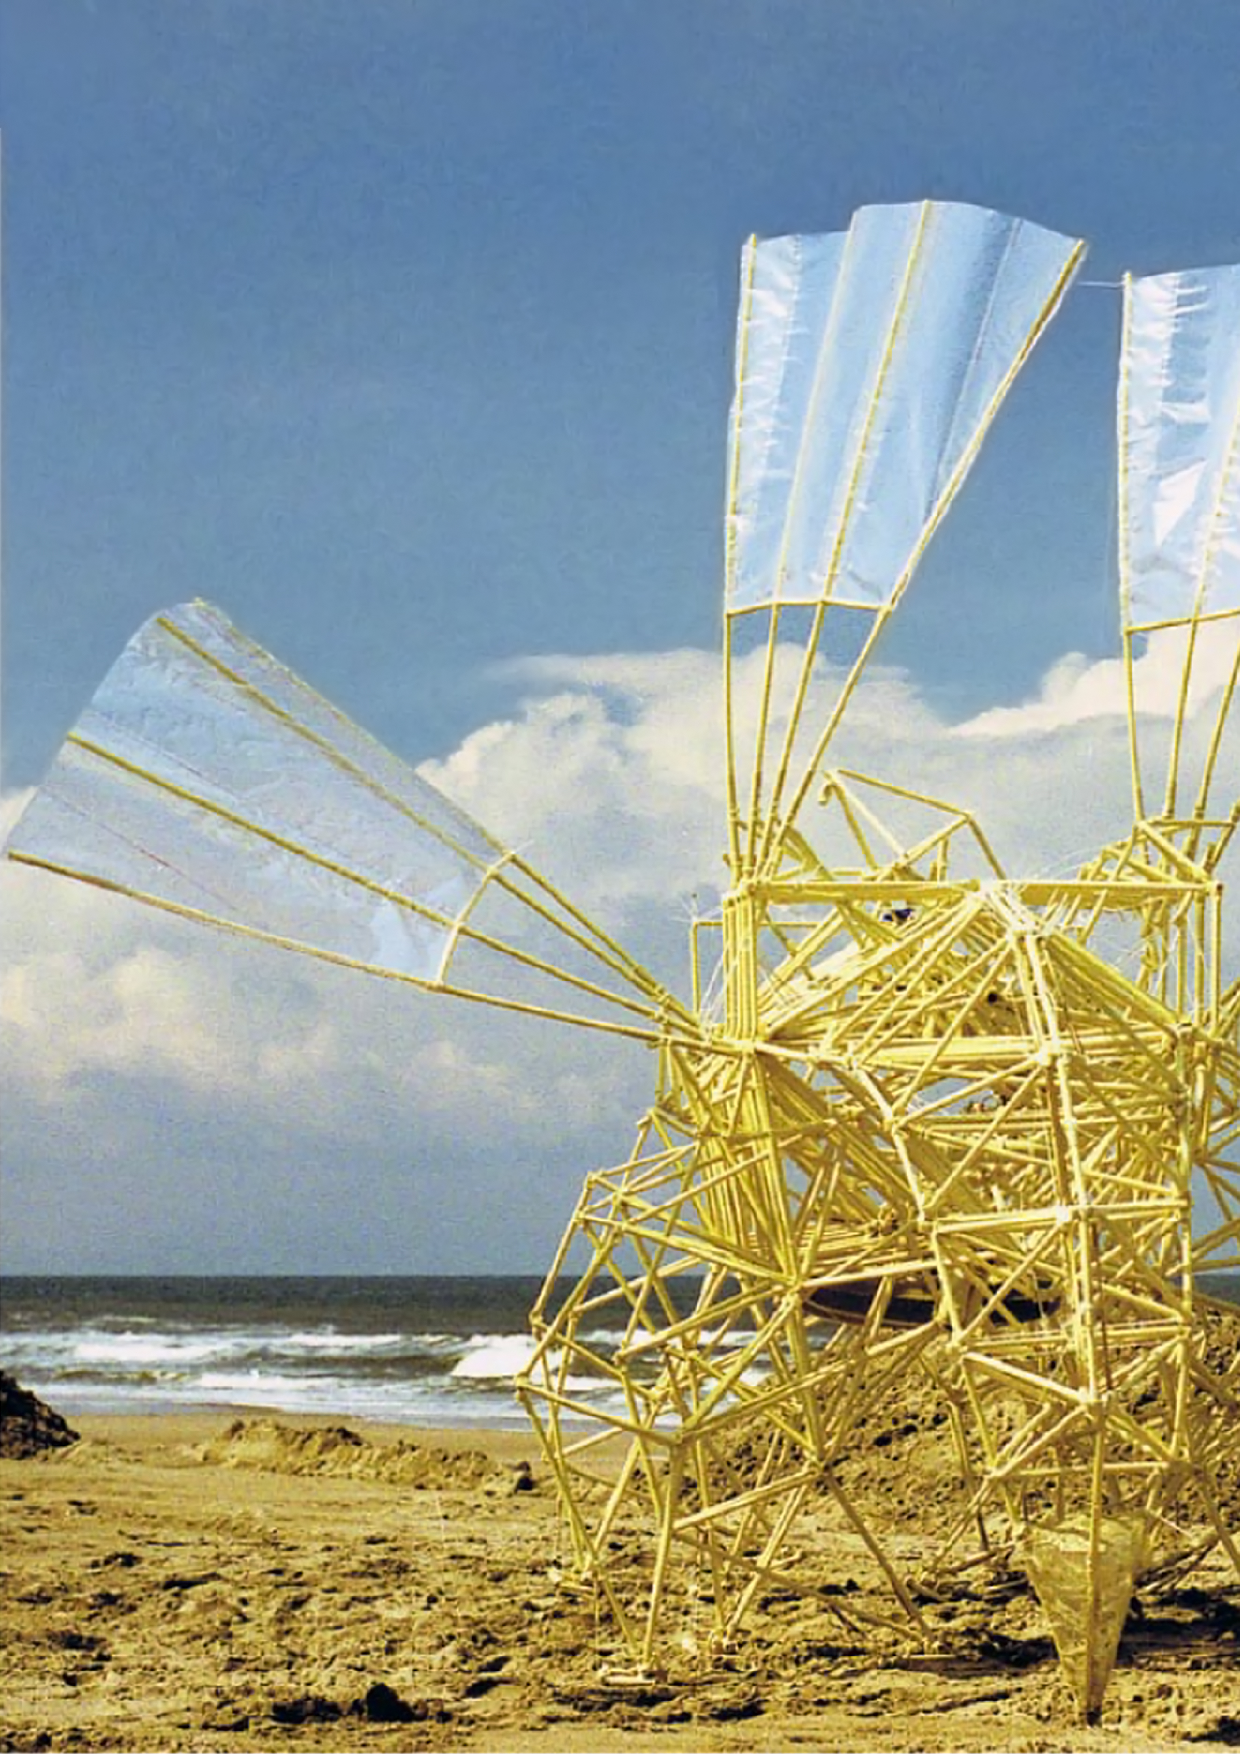
\includepdf{../media/chapter_illustration/jansen.pdf}

\chapter{Exploring robot morphology: some fascinating work} % (fold)
\label{cha:morphology-review}

\cleanchapterquote{Cognition needs a body to think}{Rodney Brooks}

\section{Introduction} % (fold)

\begin{figure}[!b]
\centering
    \subfloat[][The turtle robot.]{\label{fig:walter_robot}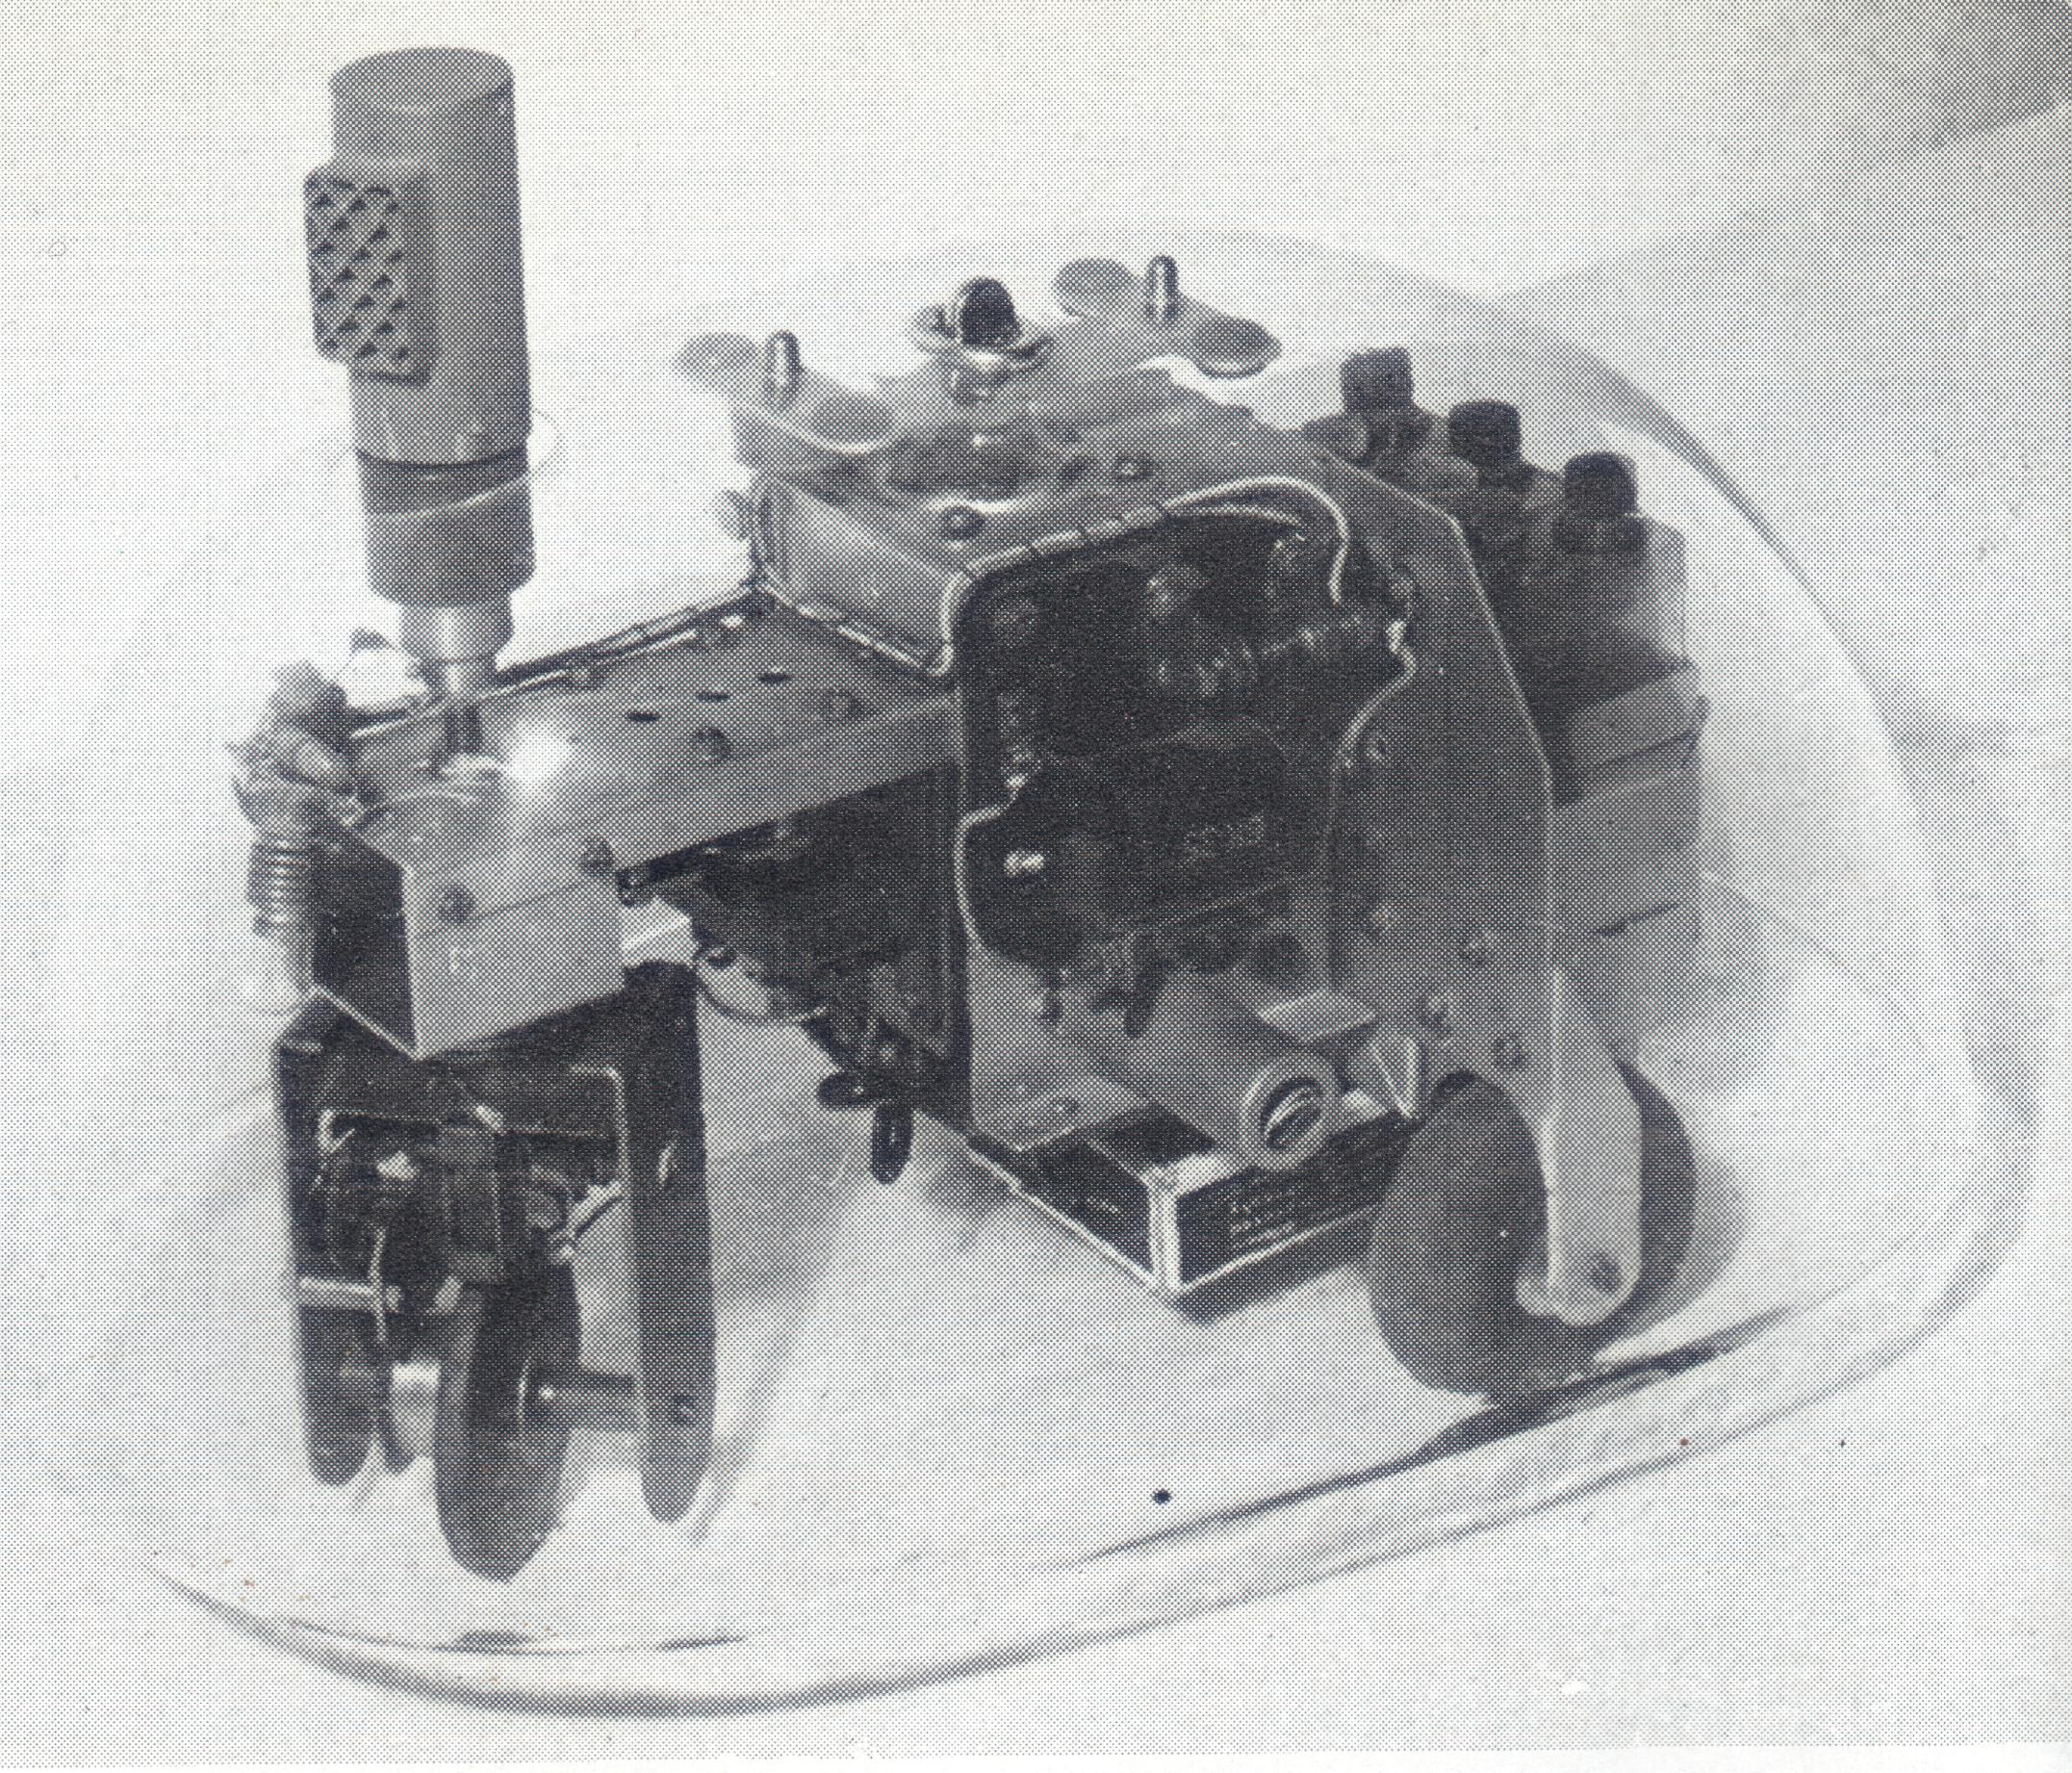
\includegraphics[height=6cm]{walter_turtoise_robot.jpg}}
    \hfil
    \subfloat[][Demonstration of obstacle avoidance behaviour.]{\label{fig:turtle_behavior}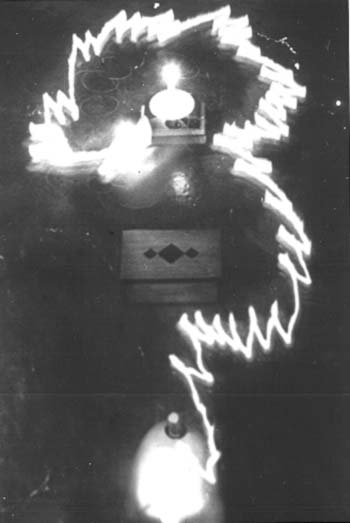
\includegraphics[height=6cm]{turtoise_behavior.jpg}}
    \caption{The W. Grey Walter's turtle was a really simple robot using a direct analog connexion between light sensors and wheel actuators. The way sensors and actuators were plugged determined the robot’s behaviour. It could demonstrate complex behaviour such as obstacle avoidance or returning to its recharging station.}
    \label{fig:turtle_robot}
\end{figure}


In 1949, Elmer and Elsie, also known as the turtle robots (see \figurename~\ref{fig:walter_robot}), created by the cybernetic pioneer W. Grey Walter, could be considered as two of the earliest robots in the era of modern robotics history (1950-now). Back at this time, the transistor had just been invented (1948)~\parencite{brinkman1997history} and calculus was done with mechanical machines. The turtle robot was entirely analog but was able to demonstrate complex behaviours (see \figurename~\ref{fig:turtle_behavior}). Without any "reflection" or internal representation of itself and the world, this robot, thanks to its mechanical design and the direct analog interaction between sensors and actuators was able to avoid obstacles and reach its charging station~\parencite{walter1950imitation}.
These complex behaviours, which can be compared to the ones found in nature, were in fact done without any kind of intelligence and were actually emerging from the interaction between the robot’s morphology (i.e. where sensors are placed and how they are connected with actuators) and the robot’s environment (i.e. light sources).


\subsection{The limits of the cognitivist approach} % (fold)


With the arrival of digital computers, researchers imagined the opening up of a field where it could be possible to replace pre-wired analog electronic behaviours by the use of computer-run programs. Not dependent on the hardware platform, robots would be therefore more versatile.
Artificial intelligence (AI) term was introduced in a workshop organized in 1956 by a MIT professor John McCarthy (REF). On the whole, participants were convinced, that by using the notion of computation or abstract symbol manipulation, it would be possible to reproduce interesting abilities similar to human ones~(\cite{kaufmann1979machines}, \cite{haugeland1989artificial}). The symbol-processing paradigm or cognitivist paradigm sees cognition as pure computation. In other words, the abstract algorithm or the program doing calculus constitutes the actual process of intelligence. Eventually, researchers following this paradigm no longer saw physical incarnation as a relevant component. Cognitive and computationalist hypotheses state that thought is reducible to a set of symbolic calculations being established~\parencite{fodor1987psychosemantics}. The body, on the other hand, is forgotten, irreparably separated from the mechanisms of intelligence~\parencite{kaplan2008corps}.
Moreover, the robot body became a handicap, which often ruined the efficiency of algorithms and programs created by AI researchers. Indeed, the real world body is non-perfect, there is some noise in sensory acquisition, there is gravity, friction and inertia acting on actuators, and the environment is always changing and unpredictable.

To overcome these issues of real world applications, the other side of the robotics community, still interested in the hardware challenges strove to design more reliable and powerful robots which can react as fast and as closely as possible to the model used for its control. To do that far more precise sensors and actuators powerful enough to overcome inertia and mechanical friction are needed. Thanks to this work on hardware, industrial robots have become increasingly fast and precise, enough so to outclass any human on certain assembly tasks.

However, even with really efficient robots, artificial intelligence failed to show results comparable with the expectations researchers and society had. Robots are able to solve incredibly complex task such as chess games or able to achieve highly precise tasks in manufacturing but require a perfectly controlled and predictable environment. Going beyond this known environment seems impossible to program and none of them are able to act fluently in the real world.
Unlike virtual worlds, the real world is challenging in various ways. It is not possible to enable omniscience: we do not access the knowledge of all world states and parameters, the measures a robot can take are limited, take time and are noisy while the action taken is always different. Finally real world states are never clearly defined as precise discrete states: "the weather is never simply good or bad"~\parencite{Pfeifer06}.

While the classical approach has known great successes  in solving abstract problems such as chess games, search engines and text processing, it has failed in the understanding of natural forms of intelligence which requires a direct interaction with the real world. This is especially the case when we consider the current state of the art for interaction with humans (natural language) or objects (grasping) and locomotion in an open environment (walking, running, riding a bicycle).

\subsection{Emergence of the embodiment paradigm} % (fold)

Stuck on these major issues that crop up when acting in the real world, a kind of crisis of artificial intelligence happened in the 1980s and the cognitivist paradigm was questioned. While some researchers in the field introduced new tools such as neuronal networks, others questioned the "cognition is computation" approach and the irrelevance of the body.
Thanks to researchers such as Rodney Brooks~\parencite{brooks1986achieving}, Rolf Pfeifer~\parencite{pfeifer2001understanding} or Luc Steels~\parencite{steels1995artificial}, a novel paradigm emerges: cognition needs a body to think. Embodied artificial intelligence rejects the symbolic approach and postulates that it is not possible to have intelligence without the body and the environment~\parencite{pfeifer2001understanding}. Rather than postulating that there is a hierarchical structure in which the brain controls the body, the new theory focuses on the interaction between the two systems, even for mathematical thinking, which we could assume to be purely abstract~\parencite{lakoff2000mathematics}.

Following this paradigm, several researchers tried to tackle challenges in which the classical cognitivist approach failed i.e. the understanding of natural forms of intelligence, which requires a direct interaction with the real world. Locomotion is a great example of a task where classical robotic approaches did not yield expected results.

Animals are incredibly skilled. Even if we consider an insect with a brain a thousand times smaller than the human one, their abilities to move in an open world is simply incomparable to the most advanced current robots. One important reason for this is that in the classical view, the ability to figure out where you are is based on detailed inner models or representations having been either programmed into the robots or learned by interacting with the environment and continuously updated. The more complex these models are, the more effort is needed to acquire the relevant data to maintain them, leading to major problems when learning tasks in highly dimensional spaces (plein de REF). Brooks even argued that intelligence always requires a body and that we should forget about complex internal representations and models of the outside world; that we should not focus on sophisticated reasoning processes but rather capitalize on the system-environment interaction~\parencite{brooks1991intelligence}~\parencite{brooks1995intelligence}. Then he started to work on insect locomotion because if we understand insect-level-intelligence it will be much easier and faster to understand and build human-level intelligence~\parencite{brooks1996prospects}.

% \textbf{TODO: petite review du boulot de brooks avec les insects}

Exploring the role of morphology and how it shapes the ways we think appears to be a fascinating open field. Indeed, exploring the interaction between body properties and cognition could lead to both a better understanding of animal behaviours (human being in particular) and to building robots more adapted and robust to an open environment with unpredictable interactions.

Thus, an interesting evolution over the last decades is the demonstration of the importance of morphology for sensorimotor control, cognition and development. The research community exploring the embodiment paradigm has grown, but surprisingly not as much as we could imagine given that the classical paradigm is failing. However, new work has appeared introducing new principles we will describe in this chapter such as morphological computation, compliance or ecological balance and emergence.

In the context of this thesis we will talk about intelligence as meaning the ability to move in a natural environment, and interact with people and objects.



\section{Exploring the role of robot morphology} % (fold)

The achievement of robust locomotion in a natural environment is one of the major current challenges for robotics researchers. For decades and it is still mostly the case, the challenge of locomotion for robotic agent was only tackled through symbolic, abstract and complex computation of internal models and representations of the world. The body is reduced to a noisy interface between the abstract algorithm and the real world.
However, if we look at nature, it appears obvious that an animal’s morphology deeply changes the way it can act in its ecological system and so it has evolved in an attempt to optimize its body properties.

For some reason, in the fields of robotics and artificial intelligence the link between the body properties and the ability for a robot to move in an ecological environment does not seem as obvious. The fact that the ability to act and achieve complex tasks is due to brain computation is so deeply grounded that it even affects the general public.

However, while we may think there are indeed calculi necessary to achieve complex tasks, there is no reason they should be explicit, with precise internal models or representations of the physical world; they could be directly done through body properties.

Therefore since the 80s, considering robot morphology, defined as \emph{any characteristic of the physical structure of the robot such as link sizes, number of links, joint characteristics, mass distribution, actuator characteristics, material properties, sensor characteristics and sensor placements}~\parencite{paul2006morphological}, novel research topics appeared exploring the role of robot body morphology in the achievement of complex tasks in the natural world, especially robot locomotion.


\subsection{Morphological computation principle} % (fold)

Introduced by Rolf Pfeifer~\parencite{pfeifer2005morphological}, the morphological computation principle states that part of the computation needed in the achievement of a given task can be done implicitly through the interaction of a physical form with the ecological niche environment.
Indeed, the morphology of a robot affects its control, because it not only determines the behaviours that can be actually performed, but also the amount of control required to achieve this behaviour correctly.

A great illustration is the achievement of flight by the airplane. Most of the control permitting the plane to fly is done by the interaction between the wings and the air. Indeed in a plane, the shape of its wings is critical. Their profile generates the lift while their shape and position determine the stability of the flight.
% Actually the control is only necessary to navigate flight between two positions.

In this way, the interactive relationship between sensory-motor apparatus, morphological properties, environment and control is of prime importance. This relationship was first observed and characterized by Pfeifer as the morphology and control trade-off ~\parencite{pfeifer2001understanding}, but the mechanisms underlying this relationship have been unclear. The fact that simple physical interactions give rise to computation indicates the theoretical possibility for the dynamics of morphology to play a computational role in the system, and thereby to subsume part of the role of control~\parencite{paulinvestigation}.


\subsection{Passive and semi-passive walking} % (fold)
\label{sub:passive_principle}

The role of morphology in robot biped locomotion has been particularly explored through the research on passive dynamic walkers~\parencite{wisse2007passive}.

Biped walking on slightly inclined planes appeared as toys in the early twentieth century. Their legs are straight and they rock from side to side to allow feet to lift off the ground. The analysis of the behaviour of such systems, purely passive, is much more recent. Indeed, an advantage of such an object is its low energy consumption. The energy supplied to the system comes from the variation of potential energy due to the slope. It compensates for the energy lost during impact.

The unipodal transfer movement is similar to a passive pendulum and arises from the correct combination of an initial pulse and coupled gravity-inertial effects. The behaviour of the walker is therefore an inverted pendulum.

In the early 90s, Tad McGeer, coming from an aeronautic background, formalizes the idea of a compass biped with free articulation by the concept of the synthetic wheel~\parencite{mcgeer1990passive}.
The dynamics of the system are formalized by an equation of motion linearized close to an average vertical position of the legs, and an equation of shock for foot/ground contact modelling energy dissipation~\parencite{mcgeer1992principles}.

\begin{figure}[tb]
\centering
    \subfloat[][]{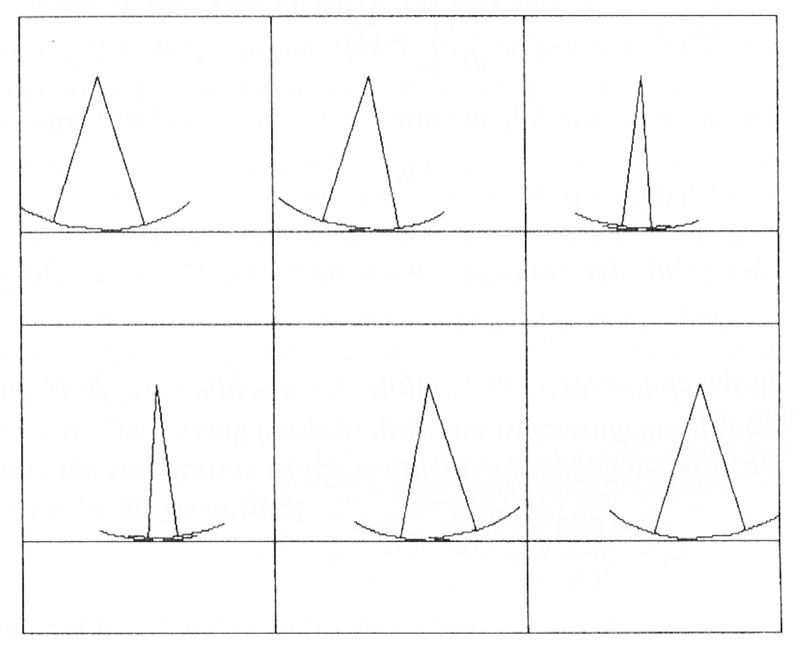
\includegraphics[width=0.4\linewidth]{simple_leg_wheel.jpg}}
    \hfil
    \subfloat[][]{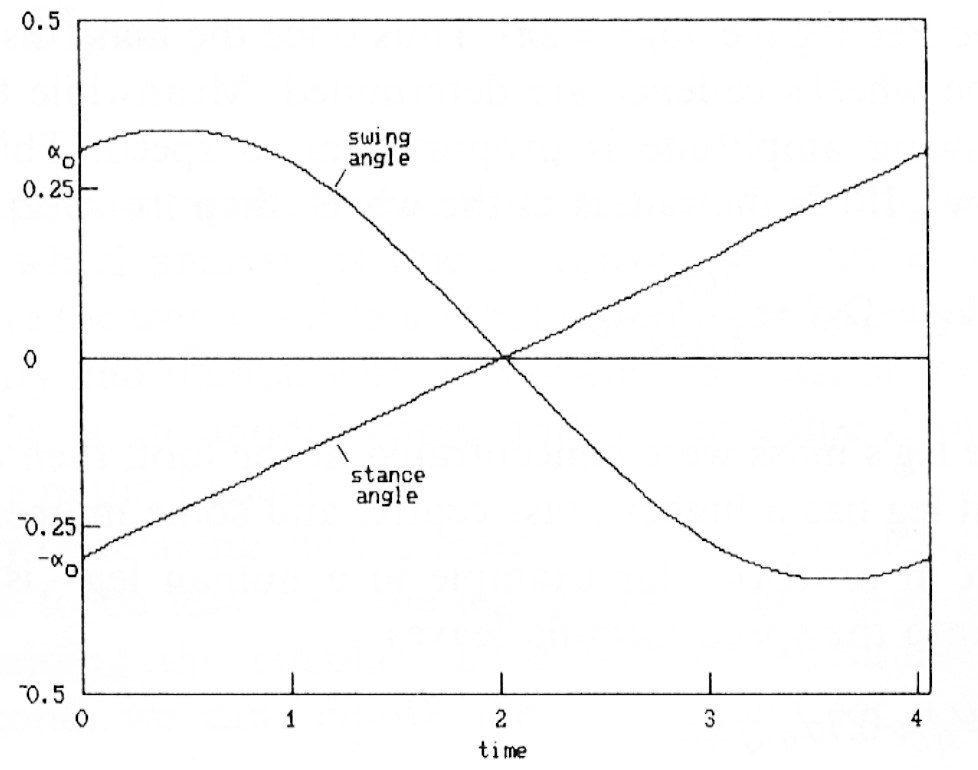
\includegraphics[width=0.4\linewidth]{simple_leg_wheel_trajectories.jpg}}
    \caption{The simplest of walking models is the synthetic wheel, a biped with straight legs and semi-circular feet (a). The stance leg rolls forward steadily like a spoke in a wheel, while the free leg swings ahead like a pendulum. Support is transferred between legs when their speeds and angles match (b). The cycle is naturally stable and will repeat continuously, thus synthesizing the motion of an ordinary wheel~\parencite{mcgeer1992principles}.}
    \label{fig:synthetic-wheel}
\end{figure}


The tuning of initial conditions conducive to passive movement is performed numerically, after one step, the robot should be back to its initial state. This model allows the robot to obtain a completely passive, cyclical walking gait (without motorization) , which is stable on a plane, slightly inclined by a few degrees. The potential energy gained during the descent exactly compensates for the energy dissipated during impact.


\subsubsection{Passive walkers} % (fold)

\begin{figure}[tb]
\centering
    \subfloat[][Tad McGeer with his prototypes]{\label{fig:tad_mcgeer}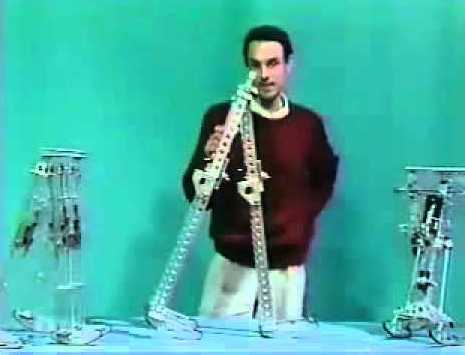
\includegraphics[width=0.49\linewidth]{tad_mcgeer.jpg}}
    \hfil
    \subfloat[][Passive walker robot]{\label{fig:mcgeer_walker}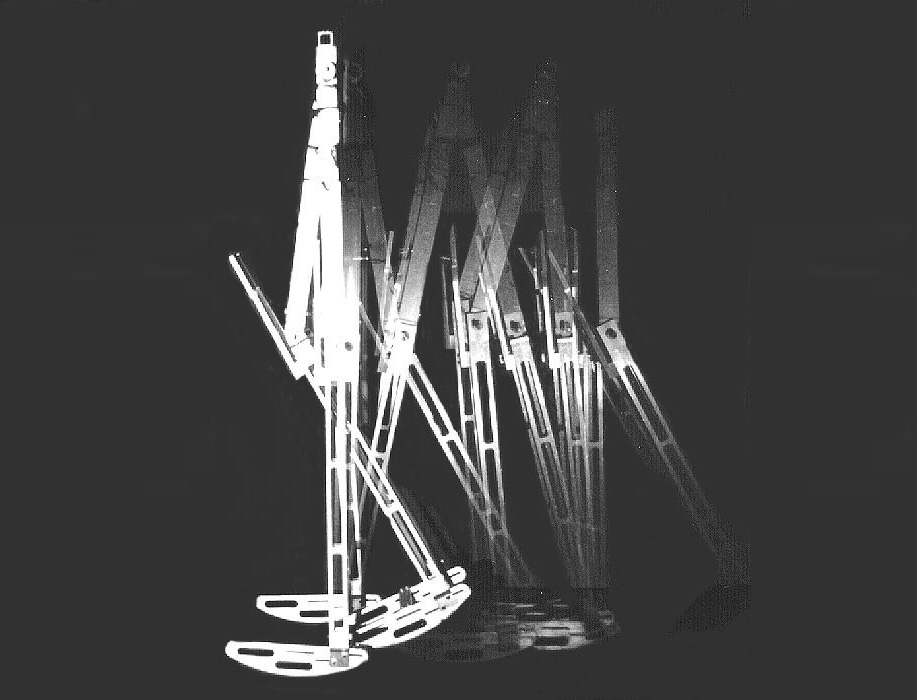
\includegraphics[width=0.49\linewidth]{mcgeer_walker.jpg}}
    \caption{Passive walker robots are just composed by mechanical elements, there is no controller nor motors, yet thanks to a clever mass repartition and feet shape, they demonstrate a very human-like and stable biped walking motion.}
    \label{fig:mcgeer_work}
\end{figure}

Tad McGeer has also showed that passive walking can be obtained on a bi-articulated robot~\parencite{mcgeer1992principles}. Appropriately shaped feet  and a judicious mass distribution generate a footstep combining a forward pendulum swinging movement on its stance leg and a swing with spontaneous flexion of the transferred leg. To make this motion possible, a device must prevent the leg from bending during the stance phase.
The dynamic behaviour is mainly determined by three dimensionless parameters: the length ratio, the mass ratio and the slope of the planar support ~\parencite{Garcia1998}.


\subsubsection{Semi-passive walkers} % (fold)
Passive robots are limited to walking on inclined ground, they cannot have a passive torso and they are locally stable robots as the domain of attraction for limit cycles is small.

\begin{figure}[tb]
    \begin{center}
        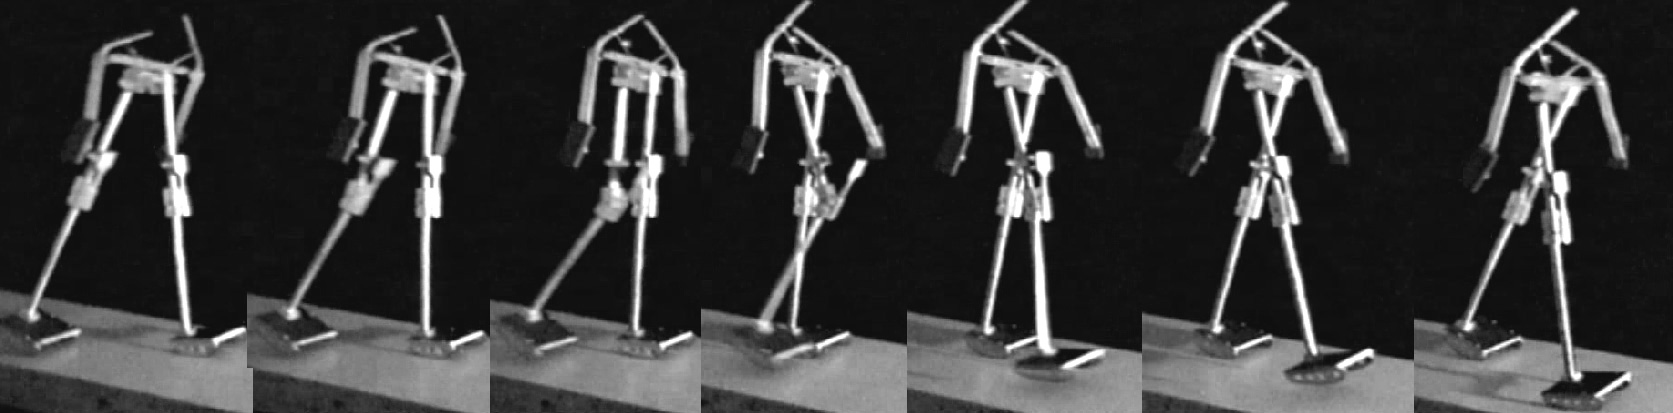
\includegraphics[width=0.99\linewidth]{cornell_biped_series.jpg}
    \end{center}
    \caption{While fully passive walker are limited to 2D walking, the Cornell walker robot created by Steve Collins~\parencite{collins2005bipedal} has demonstrated the 3D bipedal walking ability thanks to the addition of low-power actuation and arms. }
    \label{fig:cornell-biped}
\end{figure}

Thus the work on passive dynamic walkers has been pursued with the appearance of semi-passive walkers combining both specific passive properties and low power actuation to increase their robustness~\parencite{Anderson2005}. We can note the work of Collins~\parencite{collins2005bipedal} which explored the case of a semi-passive 3D biped robot. Its morphology is based on a particular mass distribution, knee locking, round feet and springs on the legs to generate an efficient walking gait while keeping its lateral and frontal balance. The concept of a 3D semi-passive robot has been pushed even further with the realization of a complete humanoid robot with torso, arms and head: the robot Denise~\parencite{wisse2005three} and Flame presented in~\parencite{Hobbelen2008} created by the Delft university.

% \begin{figure}[tb]
%     \begin{center}
%         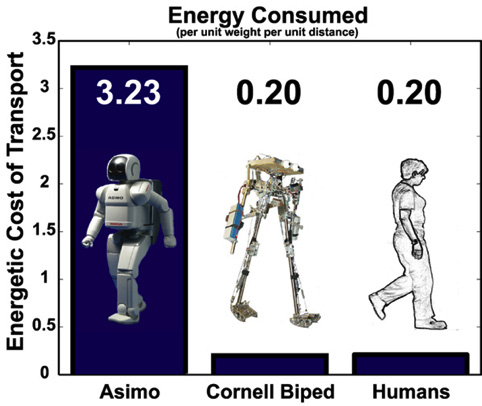
\includegraphics[width=0.6\linewidth]{comparison_cost_transport.jpg}
%     \end{center}
%     \caption{}
%
% \end{figure}


\subsection{Emergence of complex behaviours} % (fold)

Finding the rules that can lead to a desired behaviour is more difficult than explaining a real complex behaviour we can observe when an agent is interacting with its environment. Since the behaviour itself cannot be preprogramed but is always the result of an agent-environment interaction, we must design for emergence rather than directly for a specific behaviour~\parencite{Pfeifer06}. It is called the design of emergence~\parencite{Steels1991emergence}. It remains an open question how this can be done systematically. At the moment, design for emergence is rather an art than a real engineering discipline.

It is precisely in the artistic field that we find one of the most fascinating examples. Theo Jansen is a kinematic sculptor. This artist plays on the border of several fields, between engineering, research and art, is the designer of the sand beasts (see \figurename~\ref{fig:theo_jansen_beast}).

\begin{figure}[tb]
\centering
    \subfloat[][One of the Theo Jansen's creature "living" on the beach]{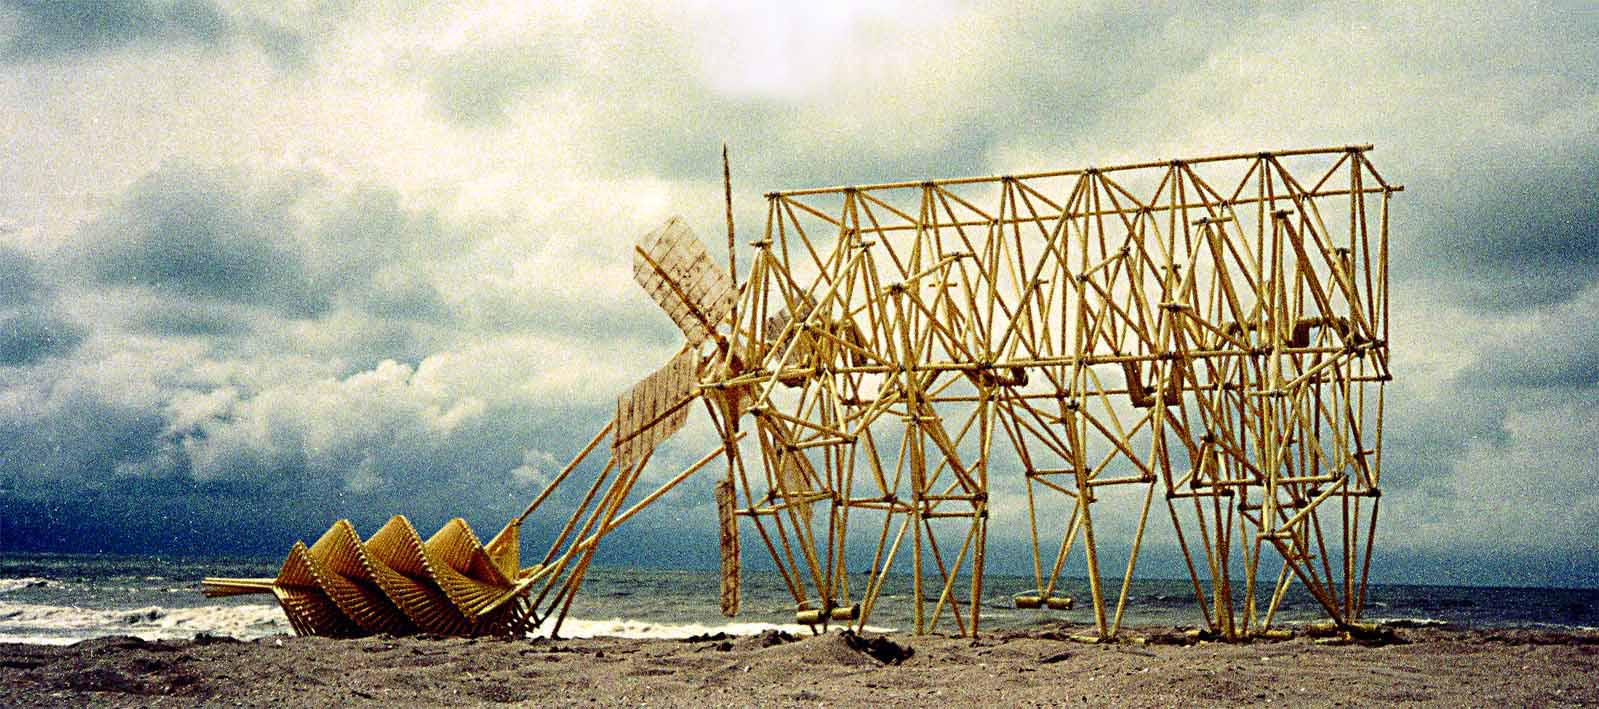
\includegraphics[width=0.99\linewidth]{theo_jansen_beast.jpg}}\newline
    \subfloat[][Leg mechanism]{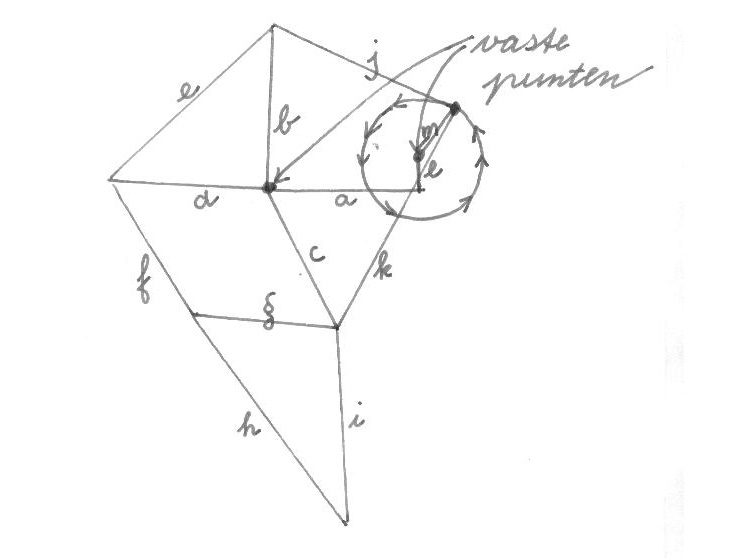
\includegraphics[width=0.32\linewidth]{strandbeest_theory.jpg}}
    \hfil
    \subfloat[][Actual trajectory]{\label{fig:jansen_leg}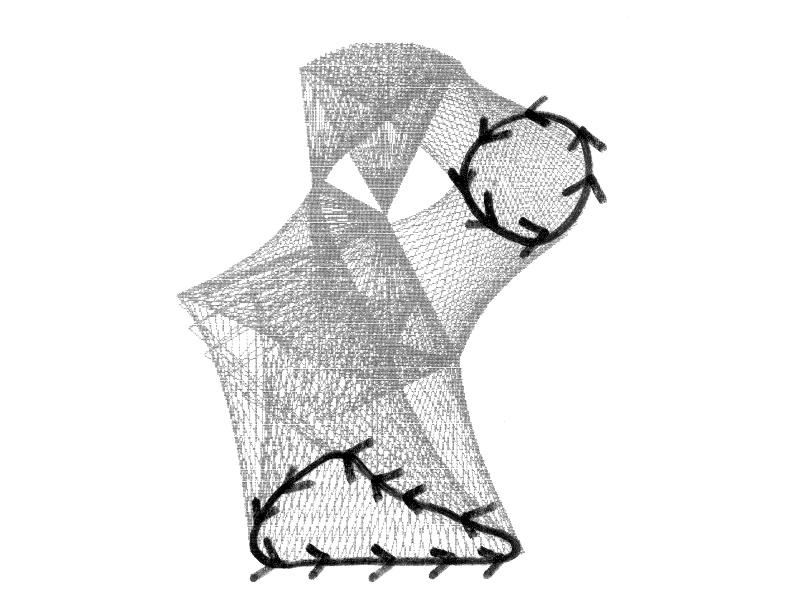
\includegraphics[width=0.32\linewidth]{strandbeest_motion.jpg}}
    \hfil
    \subfloat[][Actual leg are based on basic plastic rods.]{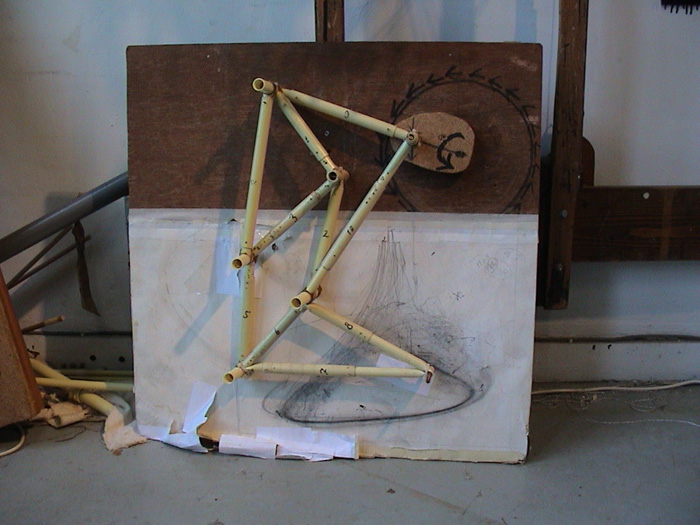
\includegraphics[width=0.32\linewidth]{strandbeest_leg_element.jpg}}
    \caption{Based on a very clever mechanism, the Theo Jansen's creature can walk robustly on terrain as complex as the beach. Moreover, he managed to add sophisticated behaviours such as avoiding the water, changing direction and store energy. As in the passive walkers robot, there is no control or motor, these behavior are only emerging from the actual morphology and the interaction with the environment.}
    \label{fig:theo_jansen_beast}
\end{figure}


These giant structures move using a really clever mechanism composed of eleven rods, the lengths of which have been tuned by numerical optimization. This system produces a walking motion(see \figurename~\ref{fig:jansen_leg}) with a center of rotation always remaining at the same level. For this reason Theo Jansen likes to say he "reinvented the wheel" but adapted to the environmental niche of his creatures .i.e. the beach.

Since the beginning of this work, Theo Jansen has created dozens of creatures that are increasingly evolved. However, the basic mechanism remains the same, both simple because it is composed of only one degree of freedom and complex because the length ratio between the eleven rods is critical and must be equal to specific numbers. Thus, using only really basic material, electric plastic tubes, Theo Jansen created multi-legged creatures capable of moving in the sand, powered by the wind~\parencite{jansen2007theo}.


The evolution of his work, led to several improvements. In this video: \url{http://youtu.be/rWbU3eV4ZpQ}, 72 legs move at the same time using one crank. But he also extended the mechanism to add independence of sorts. For instance, he added lemonade bottles to store energy. These bottles are used as pressure tanks filled using pumps powered by the wind. Beasts can utilize this stored energy in case the wind fades away.

Also, a natural enemy of these beasts is the sea. Using the same basic material, Theo Jansen created sensors able to detect water and reverse the way beasts move. The same principle allows also these beasts to avoid obstacles.

Thus the work of Theo Jansen goes beyond kinematic art and is really instructive for robotic and IA research fields. Indeed, thanks to a specific morphology adapted to their environmental niche, his creatures are able to act autonomously and "survive" in the real world. No computation, no abstraction, the apparent intelligence of these creatures comes only  from a direct interaction between their particular morphologies and the environment. Based on low cost materials, yet clever mechanisms, his work is a meaningful proof of concept showing how the morphology of an agent can lead to the creation of complex behaviour like those we could call "intelligent".


% \subsection{Bio-inspiration} % (fold)

% Toward the understanding of natural form of intelligence and the achievement of robust robotics, several researcher have been interested by insects and the animal kingdom. Indeed, it appears that nature has created a wide variety of very efficient organisms.


\subsection{Compliant robotics} % (fold)
Compliance describes the stiffness of a system. It is mostly used in robotics to describe how an actuator or a mechanical part reacts to external forces when trying to reach a position. The real output of a compliant actuator will be modified by its interaction with the environment while a rigid actuator will force the output to be the desired one. Compliance can also be achieved by the use of soft materials for the mechanical structure (also called soft robotics), whereby the link or the shape of the robot can be deformed by its interaction with the environment.

Several projects have already shown the importance of an adequately compliant morphology in achieving complex sensory-motor behaviour such as legged locomotion in complex environments with relatively little control.  This is illustrated by the quadruped Big Dog those compliance relies on hydraulic actuators~\parencite{raibert2008bigdog} as well as the RHex robot~\parencite{saranli2001rhex} using six compliant legs. Both demonstrate impressive adaptability and crossing behaviour over rough-terrain.

\begin{figure}[tb]
\centering
    \subfloat[][The Rhex robot is a compliant hexapod able to move quickly and robustly over complex terrain.]{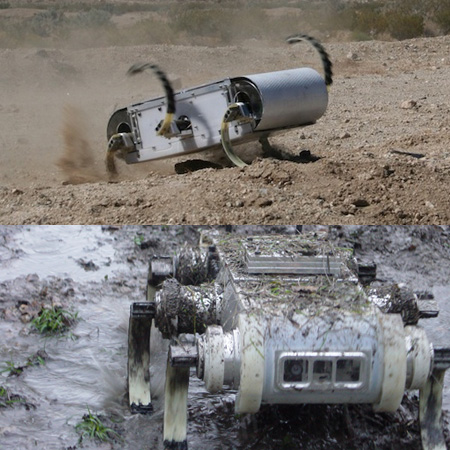
\includegraphics[height=5cm]{rhex.jpg}}
    \hfil
    \subfloat[][Raptor has both compliant actuators and feet. It is currently the fastest bipedal robot.]{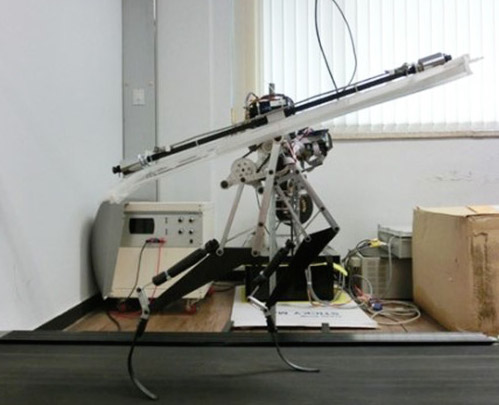
\includegraphics[height=5cm]{raptor-robot.jpg}}
    \caption{Example of robots those impressive behaviours were achieved thanks to a compliant morphology.}
    \label{fig:compliant_robot}
\end{figure}

Also certain humanoid robots have shown the importance of a compliant structure for human robot interaction. For example the compliant structure of the vertebral column and legs of Acroban~(\cite{ly2011bio}, \cite{Oudeyer2011}) was shown to permit a self-organized physical human-robot interface allowing non-expert users to lead the robot by the hand.

Furthermore, it has been shown that the compliance of the body explains the dynamics of walking and running~(\cite{Geyer2006}, \cite{iida2007bipedal},) and appears to be a key-feature toward the achievement of the fastest current robots both for quadrupedal (DARPA Cheetah robot\footnote{Darpa cheetah video: \url{http://youtu.be/d2D71CveQwo}}) and bipedal running (see Raptor robot\footnote{Raptor robot video: \url{http://youtu.be/lPEg83vF_Tw}}).



\section{Conclusion} % (fold)

Researchers have shown the interest of having a well-adapted morphology, by exploring several aspects such as morphological computation, passive dynamics or compliance with this goal in mind. In addition, we could complete this review about the role of morphology with the ecological balance principle~\parencite{pfeifer2005new}, bio-inspiration~(\cite{scarfogliero2009use}, \cite{Pfeifer07}) or the coupling of adequate morphologies with central-pattern generators that has been shown to generate robust locomotor behaviour~(\cite{ijspeert2007swimming}, \cite{steingrube2010self}).

The work presented in this chapter shows the recent awareness in the robotics field of the importance of morphology. It appears increasingly clear that the achievement of robust robotic requires an understanding of the interaction between robot morphology, control and environment.

However, as shown in the diversity of projects, the role of morphology is still a research field open to exploration. For this purpose, an abstract robot is not sufficient and it is necessary to have a real robotic platform to experiment on. This will be the subject of the next chapter, in which we will present an overview of the current robotics platforms.


